\section{The Proposed Algorithm}
\label{sec:proposed}
In this section we detail the working of our proposed \textit{MLTimer} algorithm. The \textit{MLTimer} algorithm consists of the following modules as shown in Figure~\ref{fig:algo}:
\begin{itemize}
    \item \textbf{Learning Module:} This module employs Support Vector Machines (SVM) to predict an initial configuration ($V_t$ and $size$ values) for each gate in the netlist that could ultimately lead to a power and delay optimal solution.
    \item \textbf{Delay Recovery Module:} This module takes the output configuration provided by the learning module and the target delay as inputs. The module then checks the design for any timing violations and fixes them iteratively using Algorithm~\ref{alg:delay}.
    \item \textbf{Leakage Power Recovery Module:} This module uses the solution provided by the delay recovery module to perform leakage optimization.
\end{itemize}

\noindent We now describe the working of each module in detail.

\begin{figure}[!t]
\begin{center}
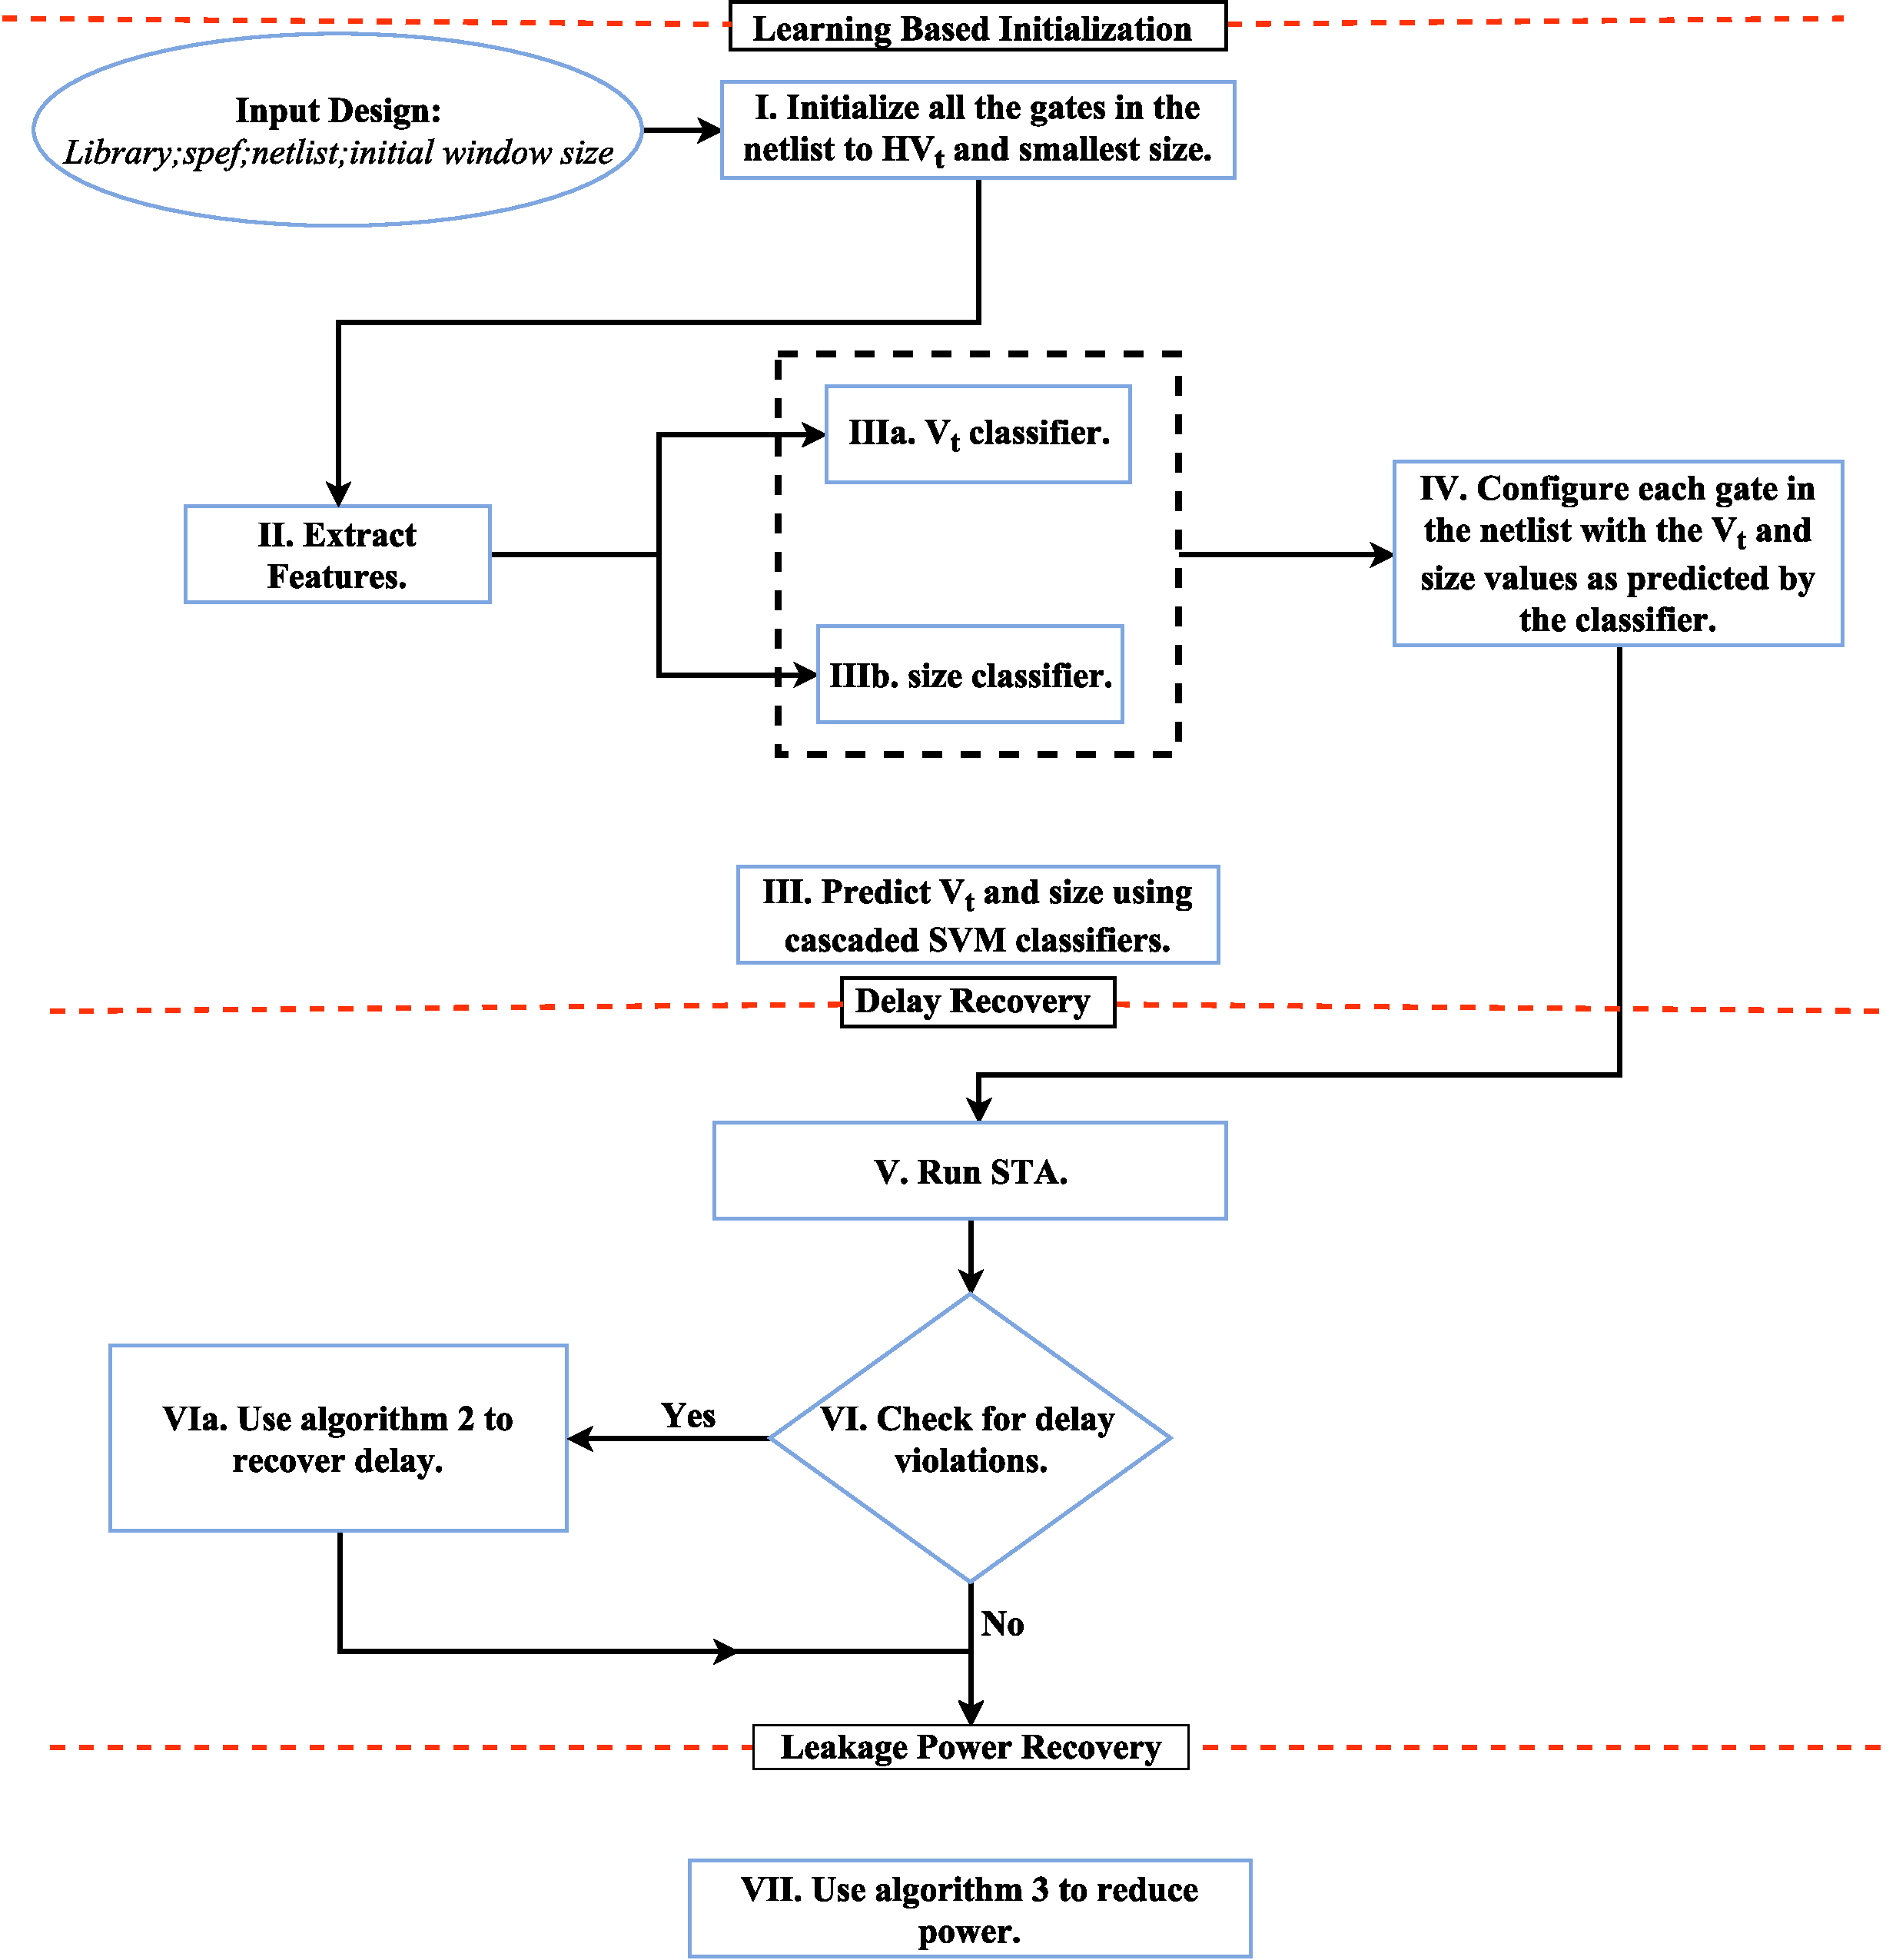
\includegraphics[scale=0.35]{Chapter3/fig/learntimer.pdf}
\caption{The flowchart describes the various steps of our \textit{MLTimer} algorithm.}
\label{fig:algo}
\end{center}
\end{figure}


\subsection{The Learning Module}
\label{sec:feature}
\noindent As seen in Figure~\ref{fig:algo}, the Learning Module takes the netlist initialized to $HV_t$%\footnote{The standard cell library has three available $V_t$ choices. We designate the largest $V_t$ choice as $HV_t$ $(V_t=2)$, the second as $SV_t$ $(V_t=1)$ and the third and smallest choice as $LV_t$ $(V_t=0)$. The largest $V_t$ choice ($V_t=2$) is slower but better in terms of leakage power whereas the smallest ($V_t=0$) is faster but consumes more leakage power. Similarly the library has ten available $size$ choices which we designate as $size=0$, $size=1$ and so on. The gate with the smallest $size$ ($size=0$) is slower but is power efficient and the gate with the largest $size$ ($size=9$) is faster but consumes more power. }
and smallest size as input and predicts a $V_t$ and $size$ value for every gate in the netlist in order to reduce the delay and power. We saw in the previous section that though two netlists are functionally different they might share several common sub-circuits as show in Table~\ref{Tab:tab1}. However, two matching gates belonging to different structurally similar sub-circuits might differ in other aspects. For example, the second circuit might have a tighter timing constraint because of which using the $V_t$ and $size$ values of the first circuit might not improve the delay or the power. Instead it might worsen the power and the delay of the second instance thereby requiring additional iterations of optimization. Enumerating all the features that affect two matching gates and comparing them is prohibitively time consuming. Machine Learning (ML) techniques help in this regard. 
\noindent The initial configuration for each gate in the netlist is predicted using the Support Vector Machines.  Support Vector Machine \cite{SVM} is a highly memory efficient supervised learning technique that is primarily used for classification and outliers detection. An SVM engine takes in the labeled training data and tries to find a separation boundary that correctly separates each data point across dimensions. Figure~\ref{fig:SVM} shows an example of the hyperplane that a typical SVM engine computes. 

\begin{figure}[!t]
 \begin{center}

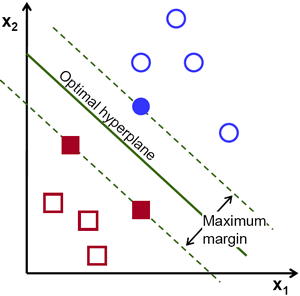
\includegraphics[scale=2]{Chapter3/fig/optimal-hyperplane}
 \caption{An example of the hyperplane/decision boundary that an SVM engine would compute. The SVM engine will take in the data-points (labeled in red and blue) $\times$ features $(X1,X2)$ and try to find the boundary between the data-points across the dimensions. Every feature accounts for one dimension.}
 \label{fig:SVM}
 \end{center}
 \end{figure}
 

 
Since SVM is a supervised learning technique, it needs to be initially trained with a labeled training data. In the first stage, we train two SVM classifiers to predict the $V_t$ and $size$ for each gate in the netlist, respectively. 
 %\subsubsection{Feature selection}
 %
\noindent We saw in Section~\ref{sec:motivation} that the final choice of $V_t$ and $size$ for a gate is not just dependent on its neighbours but on a variety of other design conditions. Hence, we identify seven such design parameters and use them as features for our technique. These features are described below:.
\begin{itemize}
    \item\textbf{  Gate Type}: This represents the functionality of the gate. Each standard cell library has a collection of low-level Boolean functions. For our experiments we use the ISPD contest library which has $13$ gate types. The gate type distribution across the benchmark circuits is shown in Table~\ref{tab:tab2}. 
 \item\textbf{ Sub-circuit}: A sub-circuit $S_i$ of a gate $g_i$ is the set of gates whose timing values are drastically affected by any change in $V_t$/$size$ of gate $g_i$.  For our experiments $S_i$ comprises the immediate fanins and fanouts of $g_i$.
 \item\textbf{ Local Negative Slack (LNS)}: We define LNS of gate $g_i$ ($LNS_i$) as the sum of all the negative slack paths that pass through $g_i$.
 \item\textbf{ Number of Fanins}: This is the number of inputs to the gate $g_i$. It accounts for the impact of modifying the $size$ of a gate $g_i$. Resizing gate $g_i$ might impact all the gates in the fanin cone of $g_i$.
 \item\textbf{ Number of Fanouts}: This is the number of gates driven by $g_i$. A gate with a large number of fanouts cannot be downscaled as it might introduce c.
 \item\textbf{  Number of Negative Slack Paths}: A high value of LNS could be because of i) a large number of negative slack paths passing through the gate $g_i$; or, ii) a small number of paths with extremely negative slack values. This feature helps to distinguish the former from the latter. 
 \item\textbf{ Slack of the Node}: As pointed out in the previous section, the amount of positive slack determines the degree to which the $V_t$ of the gate can be scaled.

\end{itemize}

 \begin{table*}[!ht]
     \caption{The Table shows the distribution of gates across the ISPD2012 benchmark suite and ShaktiC core. We use the gates from \texttt{pci} for training. In column 1, A$\times$B indicates that a gate has $A$ inputs and $B$ outputs.}
\label{tab:tab2}

     %\centering
     \begin{tabular}{|p{2cm}|p{1cm}|p{1.2cm}|p{1.8cm}|p{1cm}|p{1.6cm}|p{1.4cm}|p{1.4cm}|p{1.4cm}|}
\hline
         \textbf{Gate type}   &\texttt{pci}&\texttt{b19}&\texttt{des\_perf}&\texttt{DMA}&\texttt{leon3mp}&\texttt{netcard}&\texttt{vga\_lcd} & \texttt{ShaktiC}\\ \hline
    \texttt{NOT     }& 10,280                & 46,757        & 39,297              & 5,628         & 163,333           & 184,317           & 48,277     & 40,794        \\ \hline
    \texttt{NAND 2$\times$1}& 15,877                & 59,460        & 29,459              & 10,722        & 163,921           & 583,704           & 80,571 & 52,506            \\ \hline
    \texttt{NAND 3$\times$1}& 208                  & 6,267         & 3,930               & 372          & 8,890             & 912              & 192   & 1,387           \\ \hline
    \texttt{NAND 4$\times$1}& 295                  & 8,534         & 3,552               & 547          & 15,454            & 13,836            & 2,278 & 2,368            \\ \hline
    \texttt{NOR 2$\times$1}  & 1,403                 & 37,942        & 16,641              & 2,146         & 29,599            & 24,025            & 2,498   & 31,048           \\ \hline
    \texttt{NOR 3$\times$1}  & 14                   & 89           & 521                & 20           & 26               & 64               & 11          & 855     \\ \hline
    \texttt{NOR 4$\times$1}  & 3                    & 117          & 12                 & 1            & 1                & 6                & 2            & 1,264     \\ \hline
    \texttt{AOI21$\times$1}     & 734                  & 28,821        & 4,610               & 1,228         & 18,875            & 3,850             & 5,296   & 6,260           \\ \hline
    \texttt{AOI22$\times$1}     & 720                  & 14,921        & 919                & 1,886         & 69,817            & 48,792            & 8,449   & 14,447           \\ \hline
    \texttt{OAI21$\times$1}      & 304                  & 8,647         & 3,450               & 471          & 52,855            & 1,384             & 186    & 13,432           \\ \hline
    \texttt{OAI22$\times$1}      & 6                    & 1,119         & 36                 & 88           & 17,581            & 59               & 52       & 10,395         \\ \hline
\texttt{Total gates} & 29,844 &	212,674	& 102,427	& 23,109	& 540,352	& 860,949 &	147,812 & 174,756 \\ \hline
\end{tabular}
\end{table*}


\begin{table}[!ht]
\centering
\caption{The Table shows the percentage distribution of gates across the ISPD2012 benchmark suite and ShaktiC core. We use the gates from \texttt{pci} for training. In column 1, A$\times$B indicates that a gate has $A$ inputs and $B$ outputs.}
\label{tab:tab23}
\begin{tabular}{|l|l|l|l|l|l|l|l|l|}
\hline
Gate type ( percentage) & pci\_bridge & b19   & des\_perf & DMA   & leon3mp & netcard & vga\_lcd  & ShaktiC\\ \hline
    \texttt{NOT     }    & 34.45       & 21.99 & 38.37     & 24.35 & 30.23   & 21.41   & 32.66   & 23.66 \\ \hline
    \texttt{NAND 2$\times$1     }            & 53.2        & 27.96 & 28.76     & 46.4  & 30.34   & 67.8    & 54.51 & 30.04    \\ \hline
    \texttt{NAND 3$\times$1     }   & 0.7         & 2.95  & 3.84      & 1.61  & 1.65    & 0.11    & 0.13  & 0.7   \\ \hline
    \texttt{NAND 4$\times$1     }   & 0.99        & 4.01  & 3.47      & 2.37  & 2.86    & 1.61    & 1.54  & 1.3   \\ \hline
    \texttt{NOR 2$\times$1    }   & 4.7         & 17.84 & 16.25     & 9.29  & 5.48    & 2.79    & 1.69   & 17.77  \\ \hline
    \texttt{NOR  3$\times$1   }   & 0.05        & 0.04  & 0.51      & 0.09  & 0       & 0.01    & 0.01  & 0.49   \\ \hline
    \texttt{NOR  4$\times$1   }   & 0.01        & 0.06  & 0.01      & 0     & 0       & 0       & 0    &  0.72   \\ \hline
    \texttt{AOI  21$\times$1   }   & 2.46        & 13.55 & 4.5       & 5.31  & 3.49    & 0.45    & 3.58  & 3.58   \\ \hline
    \texttt{AOI   22$\times$1  }   & 2.41        & 7.02  & 0.9       & 8.16  & 12.92   & 5.67    & 5.72   & 8.27  \\ \hline
    \texttt{OAI 21$\times$1    }   & 1.02        & 4.07  & 3.37      & 2.04  & 9.78    & 0.16    & 0.13  & 7.69 \\ \hline
    \texttt{OAI  22$\times$1   }   & 0.02        & 0.53  & 0.04      & 0.38  & 3.25    & 0.01    & 0.04  & 5.95   \\ \hline
\end{tabular}
\end{table}

 
 \begin{table}[!ht]
     \caption{These Tables show the number of gates for each $V_t$ and $size$ in the training dataset obtained from the \texttt{pci} benchmark. It can be seen that the number of gates at $LV_t$ and $SV_t$ are much less compared to the number of $HV_t$ gates. This problem is commonly referred to as class imbalance in Machine Learning. From the fifth and sixth rows of the Table we can see that this problem exists for $size$ also.}
\label{tab:dist}

     \centering

\begin{tabular}{ll}
\begin{tabular}{|l|l|l|l|}
\hline
\multicolumn{2}{|l|}{$V_t$}              & \multicolumn{2}{l|}{Percentage of gates} \\ \hline
\multicolumn{2}{|l|}{$V_t = 0$ $(LV_t)$} & \multicolumn{2}{l|}{8.47}                \\ \hline
\multicolumn{2}{|l|}{$V_t=1$ $(SV_t)$}   & \multicolumn{2}{l|}{1.86}                \\ \hline
\multicolumn{2}{|l|}{$V_t=2$ $(HV_t)$}   & \multicolumn{2}{l|}{89.97}               \\ \hline
\end{tabular}
&
\begin{tabular}{|l|l|l|l|}
\hline
\multicolumn{2}{|l|}{$size$}              & \multicolumn{2}{l|}{Percentage of gates} \\ \hline
\multicolumn{2}{|l|}{0} & \multicolumn{2}{l|}{84.40}                \\ \hline
\multicolumn{2}{|l|}{1}   & \multicolumn{2}{l|}{13.75}                \\ \hline
\multicolumn{2}{|l|}{2}   & \multicolumn{2}{l|}{0.7}               \\ \hline
\multicolumn{2}{|l|}{3}   & \multicolumn{2}{l|}{0.7}               \\ \hline
\multicolumn{2}{|l|}{4}   & \multicolumn{2}{l|}{0.2}               \\ \hline
\multicolumn{2}{|l|}{$> 5$}   & \multicolumn{2}{l|}{0.25}               \\ \hline
\end{tabular}
\end{tabular}
\end{table}

\noindent There is no empirical/analytical technique to prove that the above features are comprehensive but they are good indicators as to what might happen to the chosen gate. For example, a gate with extremely high fanout count is highly unlikely to be downsized though it might have high positive slack because the downsizing may lead to capacitance violations. We extract these features for every gate in the netlist. We represent each gate in the netlist along with its associated features  as a matrix. In the training phase, each row in the matrix is associated with a $V_t$ and $size$ label. In the testing phase, the matrix is provided as the input to the trained SVMs that predict a $V_t$ and $size$ value for each gate in the netlist. 


% Please add the following required packages to your document preamble:
% \usepackage{booktabs}
% \usepackage{multirow}
% \begin{figure*}[!t]
%  \begin{center}

% 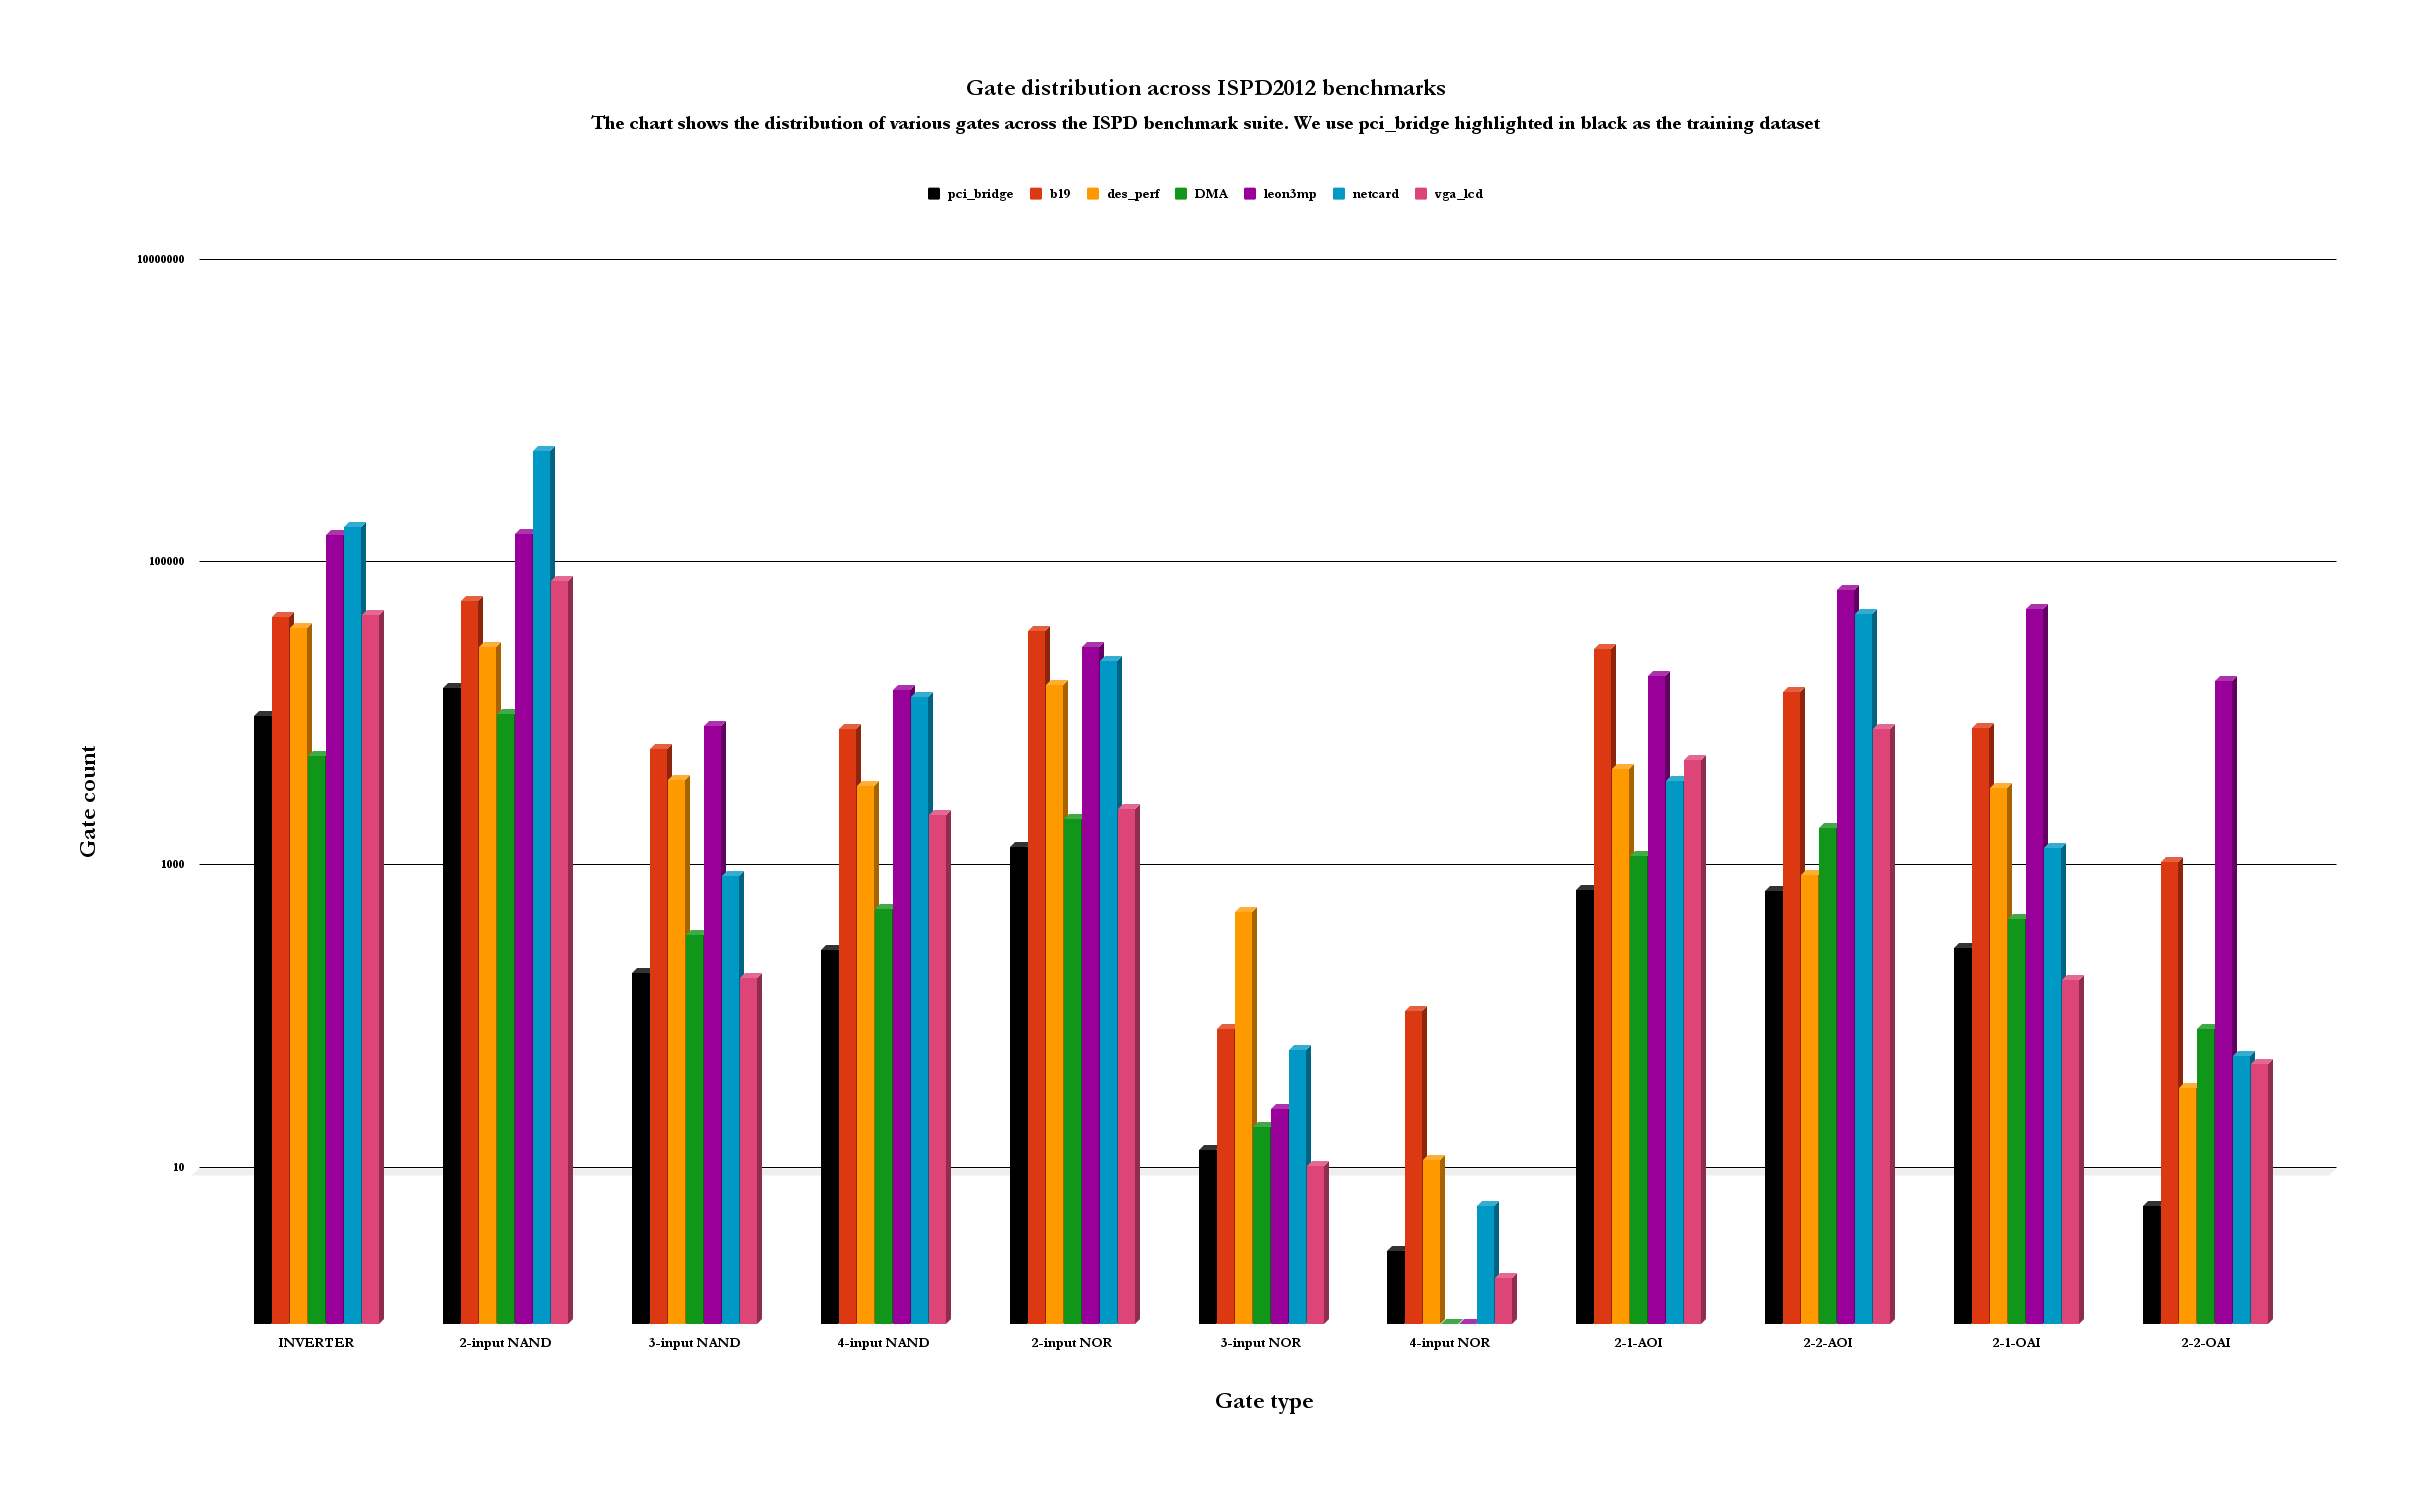
\includegraphics[scale=0.2]{fig/chart1}
%  \caption{An example of the hyperplane/decision boundary that an SVM engine would compute. The SVM engine will take in the data-points(labeled in red and blue) $\times$ features (X1,X2) and try to find the boundary between the data-points across the dimensions (one feature==one dimension).}
%  \label{fig:dist2}
%  \end{center}
%  \end{figure*}
 

% \begin{table*}[!t]
% \begin{minipage}{0.1\linewidth}
% \centering

% \begin{tabular}{|l|l|l|l|l|l|l|l|l|l|l|l|l|}
% \hline
% Gate type   & NOT & \begin{tabular}[c]{@{}l@{}}2-input\\ NAND\end{tabular} & \begin{tabular}[c]{@{}l@{}}3-input\\ NAND\end{tabular} & \begin{tabular}[c]{@{}l@{}}4-input\\ NAND\end{tabular} & \begin{tabular}[c]{@{}l@{}}2-input\\ NOR\end{tabular} & \begin{tabular}[c]{@{}l@{}}3-input\\ NOR\end{tabular} & \begin{tabular}[c]{@{}l@{}}4-input\\ NOR\end{tabular} & \begin{tabular}[c]{@{}l@{}}2-1-AOI\end{tabular} & \begin{tabular}[c]{@{}l@{}}2-2-AOI\end{tabular} & \begin{tabular}[c]{@{}l@{}}2-1-OAI\end{tabular} & \begin{tabular}[c]{@{}l@{}}2-2-OAI\end{tabular} & Total  \\ \hline
% b19         & 46757    & 59460                                                  & 6267                                                   & 8534                                                   & 37942                                                 & 89                                                    & 117                                                   & 28821                                                         & 14921                                                         & 8647                                                          & 1119                                                          & 212674      \\ \hline
% des\_perf   & 39297    & 29459                                                  & 3930                                                   & 3552                                                   & 16641                                                 & 521                                                   & 12                                                    & 4610                                                          & 919                                                           & 3450                                                          & 36                                                            & 102427      \\ \hline
% DMA         & 5628     & 10722                                                  & 372                                                    & 547                                                    & 2146                                                  & 20                                                    & 1                                                     & 1228                                                          & 1886                                                          & 471                                                           & 88                                                            & 23109       \\ \hline
% leon3mp     & 163333   & 163921                                                 & 8890                                                   & 15454                                                  & 29599                                                 & 26                                                    & 1                                                     & 18875                                                         & 69817                                                         & 52855                                                         & 17581                                                         & 540352      \\ \hline
% netcard     & 184317   & 583704                                                 & 912                                                    & 13836                                                  & 24025                                                 & 64                                                    & 6                                                     & 3850                                                          & 48792                                                         & 1384                                                          & 59                                                            & 860949      \\ \hline
% pci\_bridge & 10280    & 15877                                                  & 208                                                    & 295                                                    & 1403                                                  & 14                                                    & 3                                                     & 734                                                           & 720                                                           & 304                                                           & 6                                                             & 29844       \\ \hline
% vga\_lcd    & 48277    & 80571                                                  & 192                                                    & 2278                                                   & 2498                                                  & 11                                                    & 2                                                     & 5296                                                          & 8449                                                          & 186                                                           & 52                                                            & 147812      \\ \hline
% \end{tabular}
% \caption{This table shows the distribution of gates in each ISPD benchmark. We chose pci as it has a uniform distribution of gates. }
% \label{tab:dist2}
% \end{minipage}
% \end{table*}

We use the \texttt{pci} benchmark for generating the training data. It has approximately $30,000$ gates. We use both the slow and fast variants to generate around $60,000$ samples for training the two classifiers. We implemented a greedy replacement heuristic and used it to generate the $V_t$ and $size$ for each gate of all the benchmarks used for training and validating the classifiers. Table~\ref{tab:dist} shows the distribution of the training data-points across $V_t$ and $size$. The aim of the classifier is to predict a good initial configuration which the leakage and delay  steps can use to reach an optimal solution quickly. It is crucial to identify the right set of gates that need to be swapped in order to reach the target solution. 

Since SVM is a supervised learning process, the efficiency of the classifier is highly dependent on the number and nature of training examples. Interestingly we see from Table~\ref{tab:dist} that though the total number of examples available is quite high, the number of gates that need to be swapped from their initial configuration are few in number. These are the gates that are of interest to us as they help in identifying the conditions to swap the $V_t$/$size$ of a gate. It can be seen in Table~\ref{tab:dist} that  we only need to swap very few gates $(\approx20\%)$ to reach an optimal configuration for \texttt{pci} benchmark from which we gather our training data. As a result there are less number of datapoints belonging to $LV_t (V_t=0)$ and $SV_t (V_t=1)$ and a similar observation is also true for $size\geq1$. Thus we see that there is a skew in the nature of datapoints available for training. This skew in the dataset is referred to as \textit{class imbalance}. We resolve the class imbalance by the following two techniques:



\begin{itemize}
    \item\textbf{ Use a cascaded classifier}: Cascaded classification is an ensemble learning technique, wherein multiple instances of the classifiers are used to predict the final class label. Instead of treating the problem as a multi-class classification problem we reduce it to a binary classification problem. We construct a series of classifiers for both $V_t$ and $size$. The cascaded classifier architecture is shown in Figure~\ref{fig:vtsvm}. The cascaded classifier setup works as follows: The first stage of the classifier is trained to classify a given datapoint as $HV_t (V_t=2)$ or not $HV_t (V_t< 2)$. If a gate is classified as not $HV_t (V_t<2)$ then it is given as an input to the subsequent stage which determine if the gate is $LV_t (V_t=0)$ or $SV_t (V_t=1)$. We follow a similar procedure for building the SVM that predicts the ${size}$. The  advantage in using a cascaded setup is that the features in each stage can be fine-tuned to perform well for only a specific $V_t$/$size$ which is easier than fine-tuning the features for all the $V_t$s or $sizes$. 
    In order to determine the accuracy of the output class we use a thresholding function. The thresholding function is based on the class probability of the classifier. If the classifier assigns a class-label at random then the class probability will be approximately equal to $0.5$. A value greater than $0.5$ indicates that the predicted $V_t$/$size$ was not randomly assigned. Thus, the class probability is a good metric to determine the accuracy of the classifier. The thresholding function is a hyper-parameter that can be individually tuned for each stage in the cascaded setup. 
\begin{figure*}[!t]
 \begin{center}
 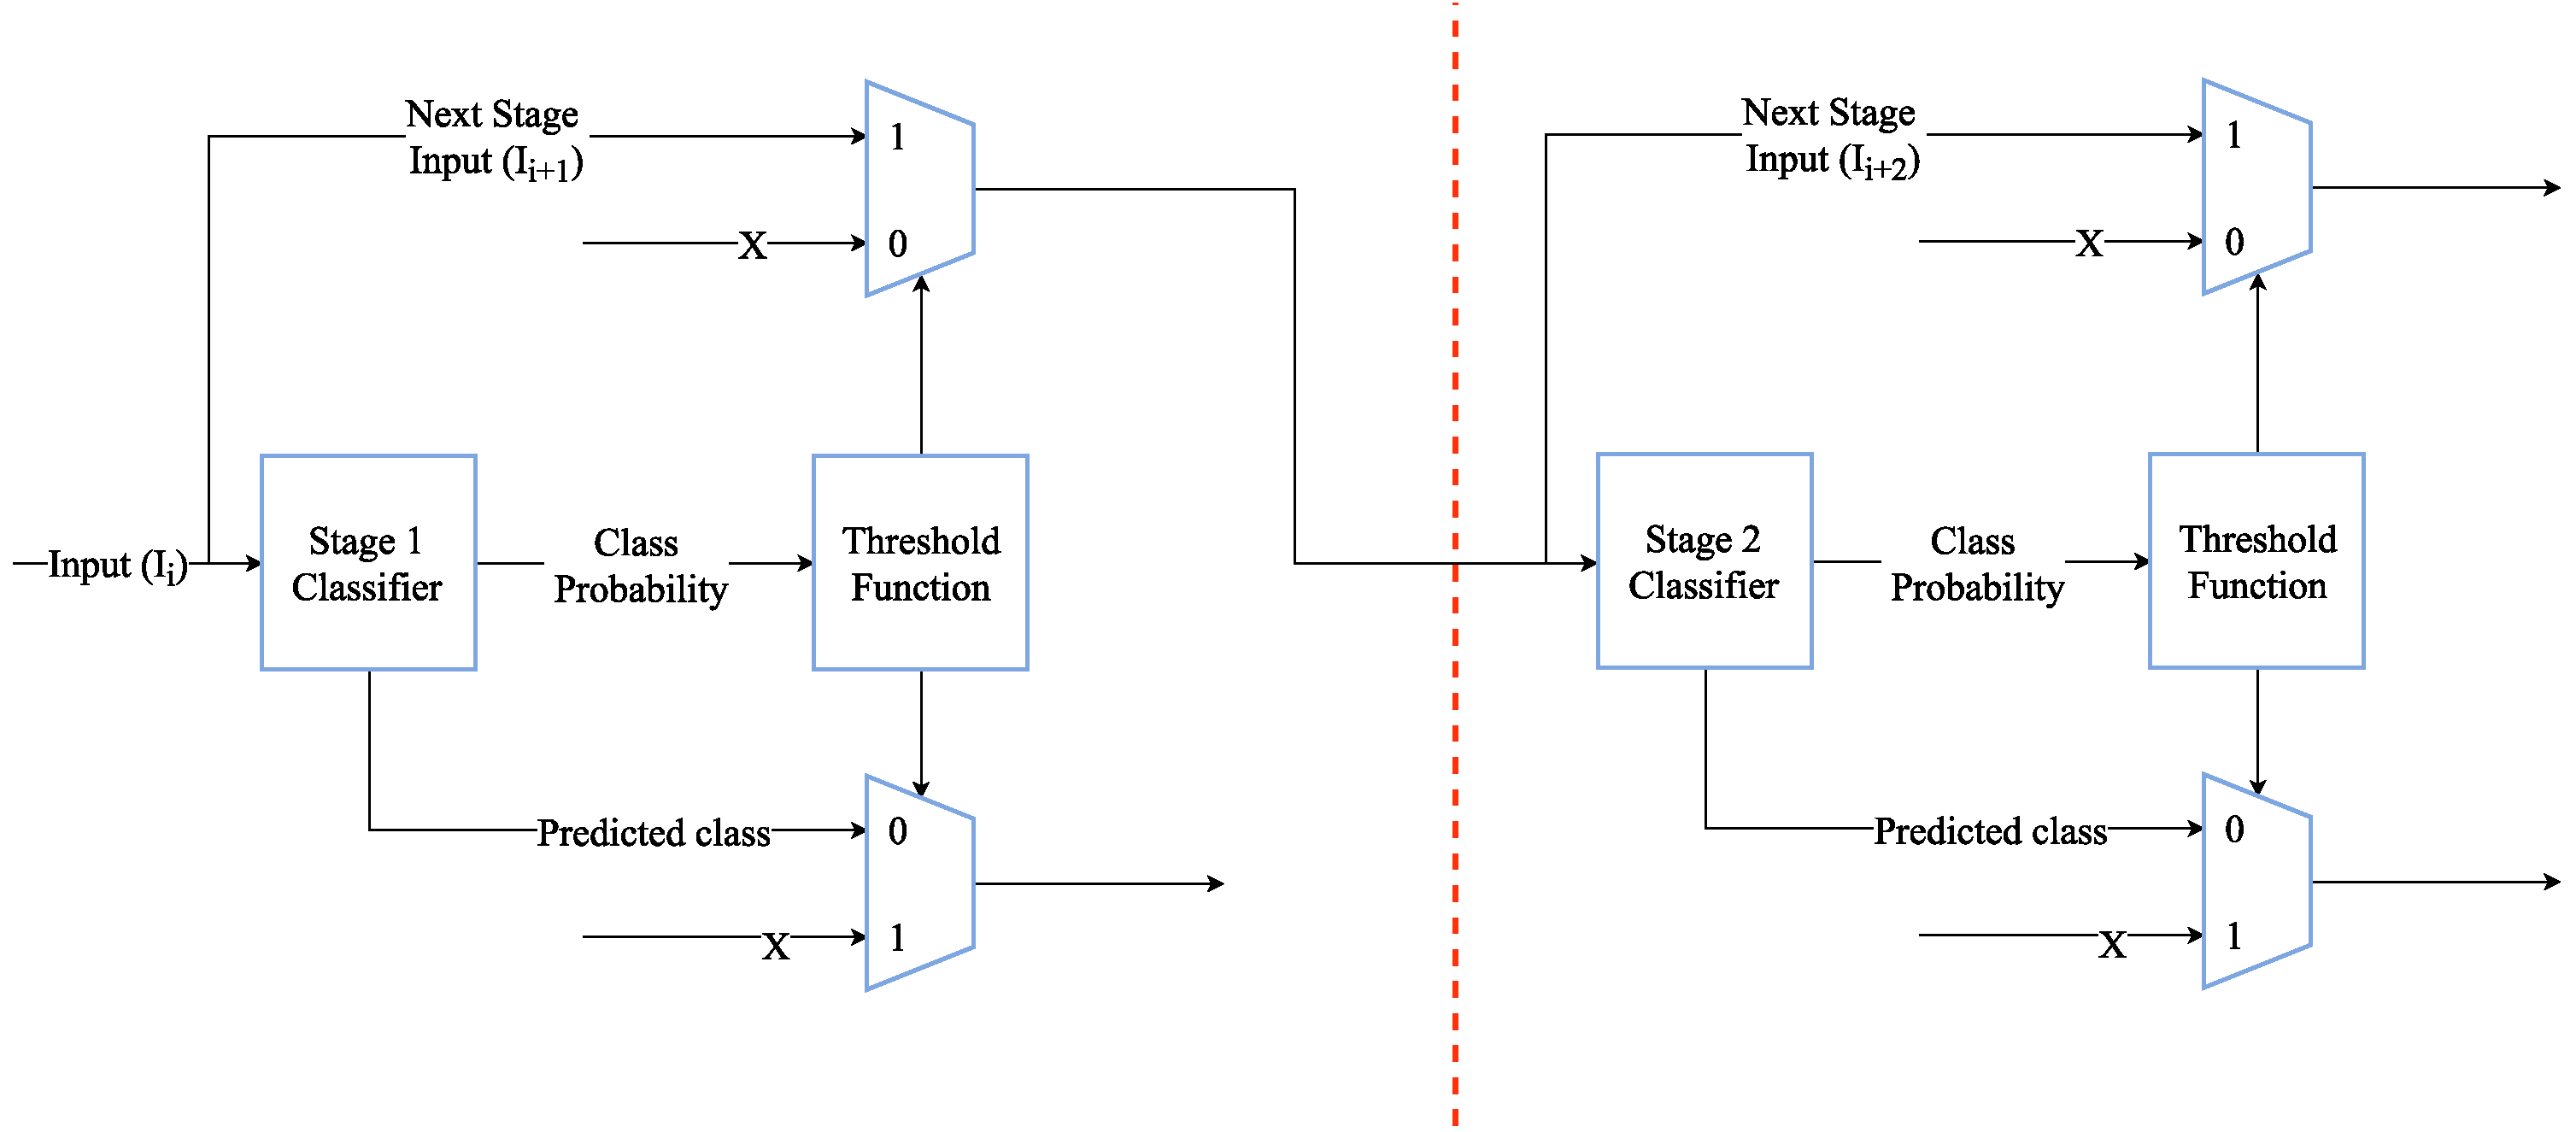
\includegraphics[scale=0.3]{Chapter3/fig/flowchart.pdf}
 \caption{Hierarchical SVM $V_t$ classifier. The first stage $V_t$ classifier classifies the points as $HV_t$ ($V_t = 2 $) or not $HV_t$ ($V_t < 2$) using the thresholding function $T_1$. If the data-point is predicted as not $HV_t$ then it is forwarded to the second stage classifier which uses the thresholding function $T_2$ to classify them as $SV_t$ ($V_t = 1$) and $LV_t$ ($V_t = 0$). The hierarchical $size$ classifier has $5$ -stages.}
 \label{fig:vtsvm}
 \end{center}
 \end{figure*}
%\begin{figure}[!t]
% \begin{center}
% 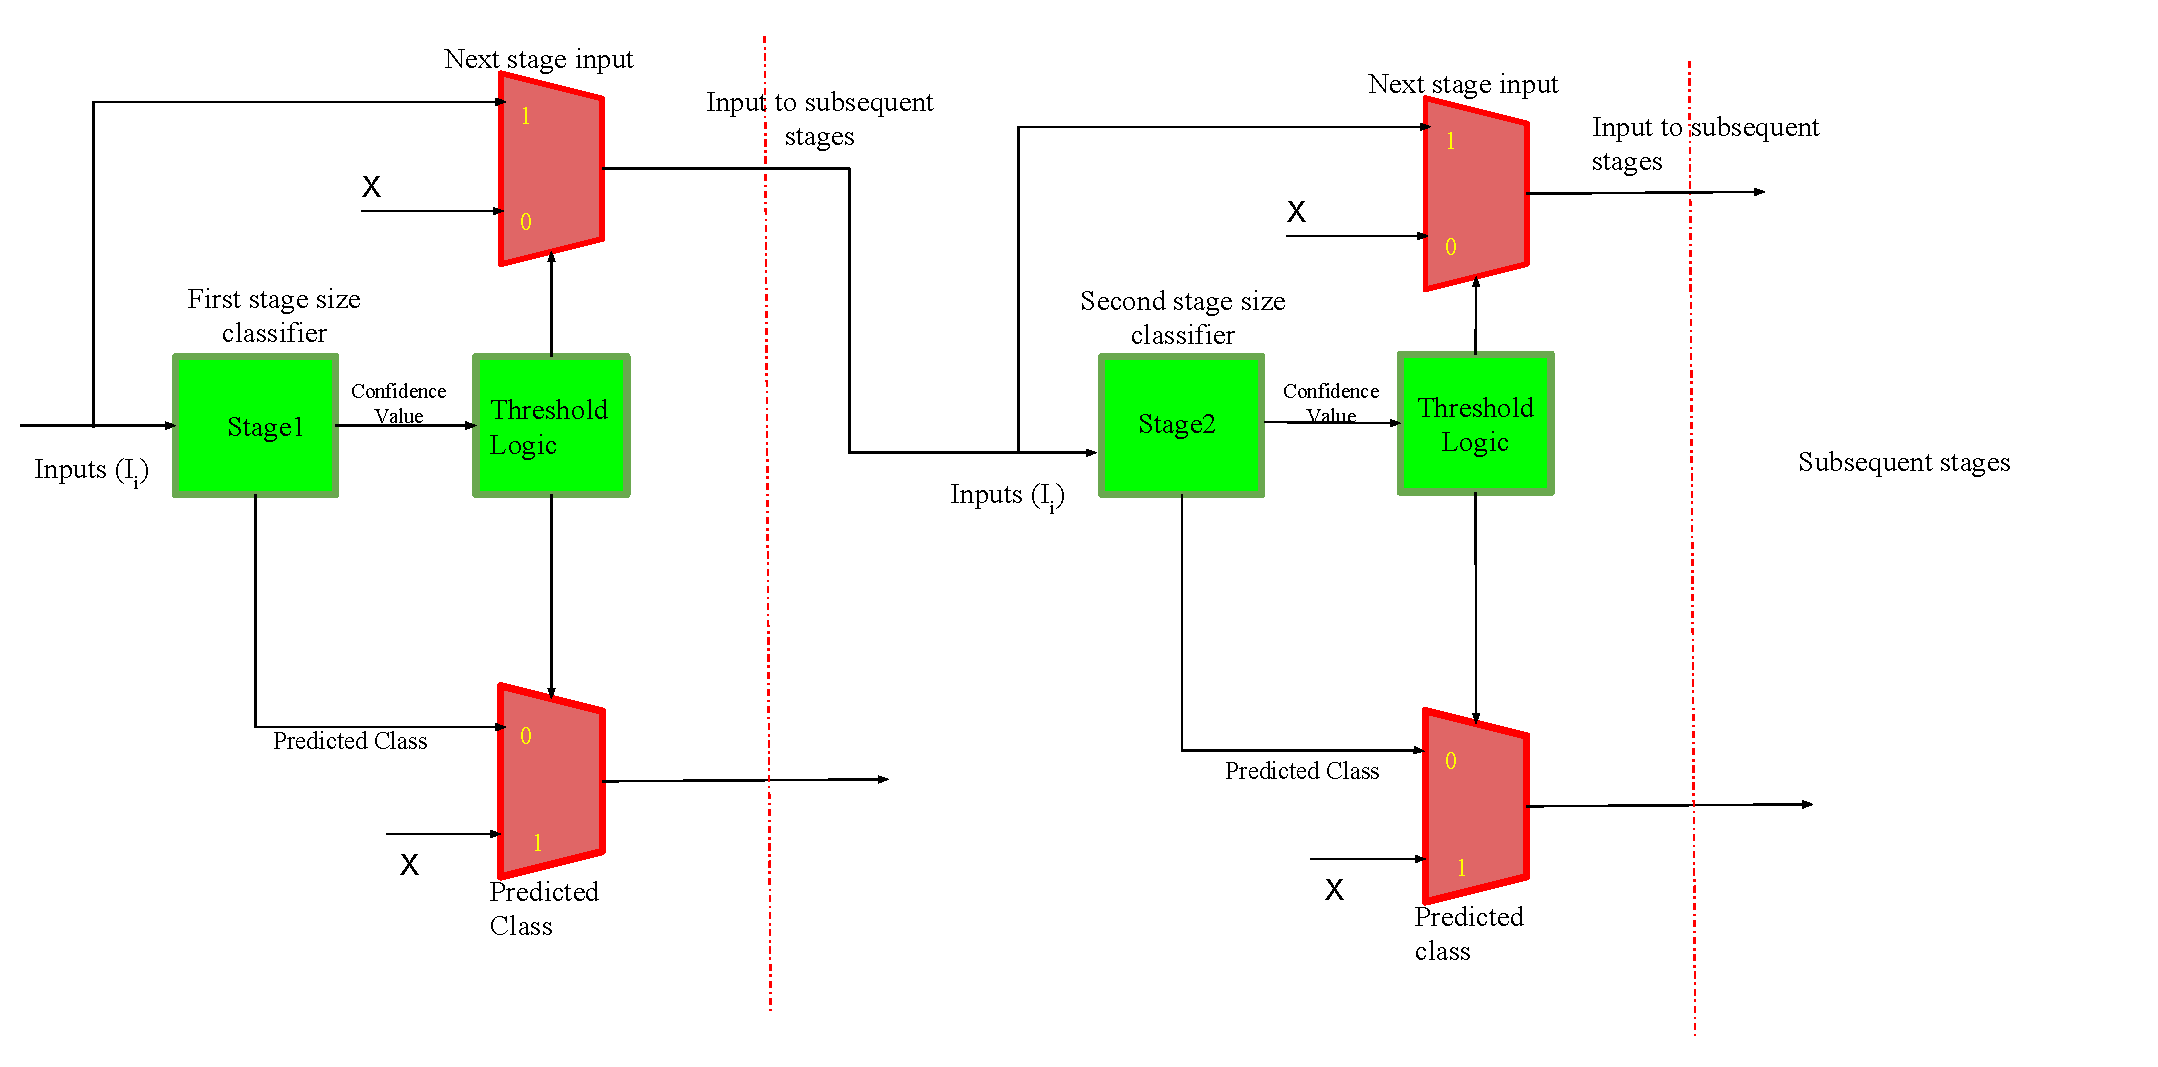
\includegraphics[scale=0.5]{fig/cascaded_size.pdf}
% \caption{Hierarchical SVM $size$ classifier. The first stage $size$ classifier classifies the points as $size = 0$ or $size > 0$ using the thresholding function. The second stage classifier takes the points labelled as $size > 0$ as inputs and uses the thresholding function to classify them as $size = 1$ and $size > 1$. The subsequent \emph{i} stages attempt to classify the input as $size=\emph{i}$ and $size > \emph{i}$.}
% \label{fig:sizesvm}
% \end{center}
% \end{figure}
    \item\textbf{ Boosting the weights of the minority classes}: While the cascaded setup solves the class imbalance problem in the $V_t$ classification, it does not completely resolve the problem in ${size}$ classification. This is because the number of sample points available for the larger sizes is extremely small as can be seen in Table~\ref{tab:dist}. It can be observed from the table that the number of sample points available for $size \geq 2$ is less than $1\%$ which is insufficient for training. This problem is resolved by boosting the weights of the features that belong to the minority classes. During training we manually increase the weights associated with the minority class to improve the performance of each classifier. 
    
  
\end{itemize}



% Please add the following required packages to your document preamble:
% \usepackage{multirow}





% \begin{table}[!t]
% \parbox{.45\linewidth}{

%    \centering

% \begin{tabular}{cc}
% \hline
% $\mathbf{V_t}$ & \textbf{\begin{tabular}[c]{@{}c@{}}Percentage \\  of gates\end{tabular}} \\ \hline \hline
% 0             & 8.47                                                                     \\ \hline
% 1             & 1.86                                                                     \\ \hline
% 2             & 89.67                                                                    \\ \hline
% \end{tabular}
%  \caption{This table shows the number of cells for each $V_t$ in the training dataset. We number the $V_t$ choices and the $size$ choices. A $V_t$ value of 0 indicates that the cell is an $LV_t$ cell while a $V_t$ value of 2 indicates that it is an $HV_t$ cell.}\label{tab:Vt}
   
% %\end{table}
% }
% \hfill
% \parbox{.45\linewidth}{
% %\begin{table}[!t]
%     \centering
%     \begin{tabular}{|c|c|}
%     \hline
%         $size$ & percentage of cells \\ \hline
%         0 & 84.40\\ \hline
%         1 & 13.75\\ \hline
%         2 & 0.7\\ \hline
%         3 & 0.7\\ \hline
%         4 & 0.2\\ \hline
%         $\geq 5$ & 0.25 \\ \hline
        
%         \end{tabular}
%     \caption{This table shows the number of cells for each $size$ in the training dataset. A cell with a $size$ value of 0 indicates that it has the smallest size possible while a cell with a $size$ value of 9 indicates that it has the largest size possible in the standard cell library.}
%     \label{tab:size}
% }
% \end{table}


% \begin{algorithm}[ht]
% %\algsetup{linenosize=\tiny}
%  \LinesNumbered`' 
% %\linesnumbered
% \title{Gateid algorithm}
% \caption{The algorithm that initializes all cells with its respective gateid}
% \label{gateid-algo}
% \KwIn{Netlist of the given circuit C containing N gates represented as a Directed Acyclic Graph (DAG) with each gate initialized to a unique prime number\footnote{The product of prime numbers is always unique and this product can be used to identify recurring sub-circuit patterns} based on gate type. }

% \For {each gate $g$ in $C$}{
%    initialize $gateid.g$ with the prime number corresponding to the gate type of g\;
%    }
%  \For {each gate $g$ in $C$}{  
%    \For{each gate $i$ in $fanins(g)$}{
%         $gateid.g = gateid.g \times gateid.i$\;
        
%         }
        
%    \For{each gate $i$ in $fanouts(g)$}{
%        $ gateid.g = gateid.g \times gateid.i$\;
        
%         }
%     }
% \KwResult{gateid is assigned to each gate}
% \end{algorithm}


%Talking points: No. of datapoints, configuration of the classifier, feature selection, 




%~\ref{learnalgo}. The algorithm has two stages \- lines ~\ref{alg:svmbegin} to ~\ref{alg:svmend} generate a good initial configuration for the netlist by using two hierarchical SVM classifiers one for $V_t$ and one for $size$. lines ~\ref{alg:delay} and lines ~\ref{alg:power} perform delay and power recovery to obtain  a leakage and power optimal configuration. 


\begin{table}[!t]
 \begin{minipage}{0.45\textwidth}
 \caption{The 2-bit prediction-based window sizing strategy adopted by {\it MLTimer}. \textsuperscript{*} The window size is incremented by a constant factor, denoted using $\alpha$.}
 \label{tab:window-sizing-strategy}

 %\begin{center}
 \centering

 %\scalebox{0.9}{

 \begin{tabular}{|c|c|c|p{4cm}|c|}
 \hline
 State & $v_{i-1}$ &$v_i$ &Description &$r(i+1)$ \\
 \hline
 $S_{00}$ &0 &0 &Timing violation in the last two iterations& $1$ \\
 \hline
 $S_{01}$ &0 &1 &Timing violation in $(i-1)^{th}$ iteration and no timing violation in $i^{th}$ iteration& $(r(i))*2$ \\
 \hline
 $S_{10}$ &1 &0 &No timing violation in $(i-1)^{th}$ iteration and timing violation in $i^{th}$ iteration& $r(i) + \alpha$ \textsuperscript{*} \\
 \hline
 $S_{11}$ &1 &1 &No timing violation in the last two iterations& $r(i)^2$ \\
 %\scalebox{0.9}{

 \hline

 \end{tabular}%}
 %\end{center}
 \end{minipage}\hfill
%\begin{figure}[!ht]
\begin{minipage}{0.35\textwidth}
 \begin{center}
 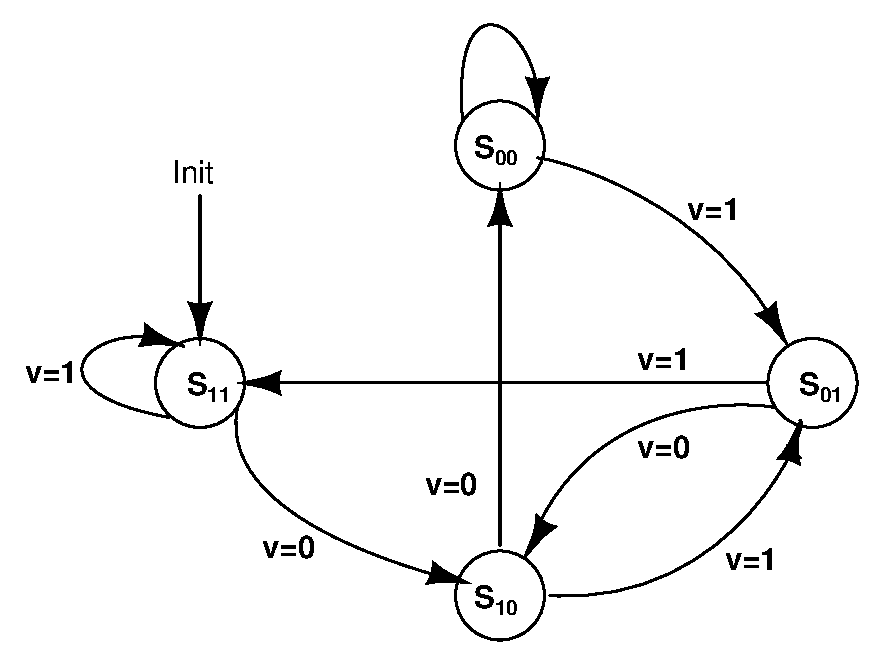
\includegraphics[scale=0.4]{Chapter3/fig/state_machine_window_sizing}
 \captionof{figure}{Transition diagram for the 2-bit prediction scheme adopted by {\it MLTimer}}
 \label{fig:state-machine-window-sizing}
 \end{center}
\end{minipage}
\end{table}


\begin{algorithm}
%\algsetup{linenosize=\tiny}
  \scriptsize
\LinesNumbered
\title{Delay Recovery Algorithm}
\caption{Delay Recovery Algorithm }
\label{alg:delay}
\KwIn{1. Netlist of the given circuit C containing N gates represented as a Directed Acyclic Graph (DAG),2. $V_t$ and $size$ values predicted by the Learning module,3. the multi-$V_t$ standard cell library and 4. the target frequency $F$.}
    \KwOut{Netlist running at the target frequency $F$.}
 $r = r_{init}$\; 
  $state\leftarrow S_{11}$\;
 $N \leftarrow gate\ count$\; 
    Initialize all the gates in $C$ with the corresponding $V_t$ and $size$ values predicted by the SVM engine. If the learning module is not able to predict a $V_t$/$size$ for a gate initialize them to a power optimal configuration $(V_t=2/size=0)$\; 
  Run STA and compute slack for each gate\; 
    \textit{cost function } $=\frac{\delta delay \times slack}{\delta leakage \times \# paths} $\; 
    For each $g_{j}$ ($1 \le j \le N$),\\ \ \ \ \  compute the cost of decreasing the $V_t$, increasing the $size$, and both\; 

 %cost of replacement \leftarrow $\frac{ $ \delta leakage \times slack$ }{$\delta delay \times paths$}$ \;
 A $\leftarrow$ list of replacements sorted in increasing order of \textit{cost function}\;  
%  \tcc{Note that all gates have slack value $\ge$ 0} 
  \While{A not empty}  {
    Take the top $r$ replacements ($A_{1}, A_{2} \ldots A_{r}$) in $A$ \; 
%  \tcc{Local validation}
     For each $A_{j}$ ($1 \le j \le r$),\\ \ \ \ \ Replace $A_{j}$ with its next high performance version (decrease $V_t$ or increase $size$) if $A_{j}$ has positive slack\; 
%  \tcc{Global validation}
      Perform a full STA on C\; 
      \If{ delay violation} {undo all the replacements done in step 12\;
    If $r \leftarrow 1$ mark $A_{j}$ as critical and delete it from A\;
      Update the state as per Figure~\ref{fig:state-machine-window-sizing}\; 
      Update the value of $r$ as per Table~\ref{tab:window-sizing-strategy}, for the new value of state\; 
    }

      \Else {
        Compute the new cost for the committed gates\;

      Update the state as per Figure~\ref{fig:state-machine-window-sizing}\; 
      Update the value of $r$ as per Table~\ref{tab:window-sizing-strategy}, for the new value of state\; 
  }
    }
\end{algorithm}




%write delay and leakage recovery module.
 
\subsection{Delay Recovery Module}
The performance of the learning module is highly dependent on the number and distribution of examples provided during the training phase. An SVM engine might under perform because of improperly chosen features, class imbalance in the dataset or less number of training examples. One or more of the above factors could lead to false positives and false negatives. These false positives and false negatives could lead to delay violations. We use Algorithm~\ref{alg:delay} to fix the timing violations in the circuit.
As seen in Figure~\ref{fig:algo}, Algorithm~\ref{alg:delay} fixes all the delay violation to ensure that the performance of the given circuit $C$ meets the target frequency. Algorithm~\ref{alg:delay} fits into the template of the iterative greedy algorithm described in Algorithm~\ref{alg:naive} except that multiple gates are replaced in each iteration of the algorithm (line 7 of algorithm~\ref{alg:naive} versus line 11 of algorithm~\ref{alg:delay}). The cost function in line 6 of algorithm~\ref{alg:delay} employed is the same as that in~\cite{hu:12}.

Algorithm~\ref{alg:delay} describes the functionality of the delay recovery module. The algorithm adaptively varies $r$ across each timing update. The value of $r$ is varied within a range $[r_{low}, r_{high}]$.In this algorithm, we initialize $r$ to $r_{low}$ and increment the same after each timing update depending on the $state$ of the timing update, until $r$ reaches $r_{high}$. After $r$ reaches $r_{high}$, it is not incremented further. In the experiments reported in this paper, the value of $r_{high}$ is fixed at $\frac{N}{2}$ ($N$ is the number of gates) based on the profiling done to find the effect of varying $r$ on the algorithm run-time for various benchmarks. Let $r(i)$ denote the value of $r$ in iteration $i$. The state transition diagram shown in Figure~\ref{fig:state-machine-window-sizing} in conjunction with Table~\ref{tab:window-sizing-strategy} describe how the value of $r$ is changed across iterations. The states in Figure~\ref{fig:state-machine-window-sizing} are defined in Table~\ref{tab:window-sizing-strategy}. Let $v(i)$ be set to $1$ if there is no timing violation in iteration $i$ else it is set to $0$. Thus the state machine will be at $S_{v_{i-1},v_i}$ at the end of iteration $i$. For example, if there was a timing violation in both iterations $i-1$ and $i$, the state machine will be in $S_{00}$ at the end of iteration $i$. Table~\ref{tab:window-sizing-strategy} describes the change in the value of $r$ in iteration $i+1$, $(r(i+1))$; that depends on the state in iteration $i$. For example, if the state at iteration $i$ is $S_{10}$, then the value of $r(i)$ is incremented by a small factor $\alpha$ in the next iteration $(r(i+1)=r(i)+\alpha)$. 
 
% The state transition We describe the way $r$ varies using the state transition diagram shown in Figure~\ref{fig:state-machine-window-sizing} and the value of $r$ at the end of every timing update is given in Table~\ref{tab:window-sizing-strategy}. It can observed from this transition diagram that $state$ in timing update $i$ can be represented as $S_{v_{i-1},v_i}$, where $v_{i-1}$ and $v_{i}$ are binary digits that denote the status of $(i-1)^{th}$ and $i^{th}$ timing updates respectively. Here, a status ($v$) of $0$ denotes the occurrence of a timing violation while a $1$ denotes a successful timing update.
 
From our experiments, we observe that the iterative correlation was very high for the first few timing updates. This implies that maximum number of gates should get replaced during those timing updates, and hence the initial state is set to $S_{11}$, which quadratically scales the window size in successive timing updates. The value of $r_{low}$ is set to $2$. A successful timing update at the end of the first iteration would cause the state to remain at $S_{11}$ while increasing $r$ quadratically to $4$, and a timing violation would cause the state to change to $S_{10}$, causing $r$ to be incremented by a small positive constant $\alpha$. A timing violation in the second update would set the state to $S_{00}$ and the window to $1$. This explains the adaptive window sizing procedure. As shown in Figure~\ref{fig:ropt} replacing $r_{opt}$ number of gates gives the best speed-up possible. However, $r_{opt}$ varies across each timing update. Ideally replacing $r_{opt,i}$\footnote{$r_{opt,i}$ is the optimal window size for the $i^{th}$ update.} gates for each of the $i$ timing updates will result in the best possible speedup. However, the value of $r_{opt,i}$ cannot be precomputed. From our initial experiments we observed that $r_{i+1}$ is strongly related to the outcome of the previous timing updates. By taking into account the outcome of the last $k$-timing updates, the likelihood of obtaining the $r_{opt}$ for the next timing update is maximized. In our setup we use a 2-bit state based sizing scheme. 
\noindent We observed that there is no significant improvement for large values of $k$. This is because the algorithm takes a large amount of time to recover from a suboptimal window size or to get to the optimal window size for a given iteration. We define this phenomenon as inertia. Consider the following scenario. If the current window size is $r_{high}$ and there is a timing violation. The number of iterations required to identify the gate causing the timing violation is $2$. However, for a large value of $k$ this increases thereby causing the algorithm to spend significant amount of time on useless timing updates. 


%\noindent We use Algorithm~\ref{alg:delay} to fix the delay violations in the circuit. We initialize the gates in netlist with $V_t$ and $size$ values predicted by the classifiers. We run an initial STA and identify the target gates using the same cost function defined in ~\cite{hu:12}.  Recovering the delay of gate $g_{i}$ will impact the other gates in the fanin/fanout cone of $g_i$. The chosen cost function computes the impact of a change in the $V_t$ or $size$ of a gate on its neighbours by computing the change in slack across all the gates in the fanin and fanout cone of $g_i$ denoted using the term $\delta delay$ in the cost function. A gate with large number of fanins/fanouts might have significantly high $\delta delay$, hence we also take into account the number of negative slack paths passing through the gate $g_i$ using the term $\#paths$. The term $\delta leakage$, which accounts for the change in leakage due to the replacement, prohibits the gate from trading off significantly large amount of power in order to improve performance.

Each execution of the \textbf{while} loop corresponds to one update interval. During each  update interval we do the following:
\begin{itemize}
\item We compute the cost of decreasing the $V_t$, increasing the $size$ and both for every gate and add them to a list \textit{A}.
\item The first $r$ choices in the decreasing order of their cost are replaced.
\item We then check for any timing violations by running a full STA. We do not use an incremental STA because running timing analysis for each gate in the window, would impose significant runtime penalty for large window sizes, ultimately offsetting the speed-up obtained by postponing the timing analysis.
\item If there is a delay violation, undo all the replacements 
\begin{itemize}
\item if $r$ is $1$, then mark the corresponding gate as critical so that it cannot participate in any further timing optimizations.
\item Update $state$ and compute new value of $r$.
\end{itemize}
\item If the timing evaluation is successful
\begin{itemize}
    \item Compute the new costs for the gates that got committed. If the gates cannot participate in further updates (gates have reached lowest $V_t$ or $size$) mark them as critical and remove them from A.
\item Update $state$ and compute the new value of $r$.
\item if value of $r$ is greater than A, then we resize $r$ to $\frac{A.size}{2}$.
\end{itemize}

\end{itemize}

\begin{algorithm}[!t]
%\algsetup{linenosize=\tiny}
  \scriptsize
 \LinesNumbered
 \title{The {\it Leakage Power recovery } algorithm}
 \caption{The Leakage Power recovery algorithm}
 \label{exponential-algo}
\KwIn{1. Netlist of the given circuit C represented as a Directed Acyclic Graph (DAG) running at target frequency $F$,2. initial window size ($r_{low}$) and upper bound on window size ($r_{high}$) and 3. a multi-$V_t$ standard cell library.}
\KwOut{The leakage optimized netlist running at target frequency $F$.} 
  $r = r_{low}$\; 
  $state\leftarrow S_{11}$\;
 $N \leftarrow gate\ count$\;
  Run STA and compute slack for each gate\;
    \textit{cost function} $=slack$\;
 A $\leftarrow$ list of gates with non-zero slacks, sorted in descending order of \textit{cost function}\; 
%  \tcc{Note that all gates have slack value $\ge$ 0} 
  \While{A not empty}  {
    Take the top $r$ gates ($g_{k_1}, g_{k_2} \ldots g_{k_r}$) in $A$ \;
%  \tcc{Local validation}
     For each $g_{k_j}$ ($1 \le j \le r$), replace the gate with its next power optimal version  (increase $V_t$ or decrease $size$) if gate $g_{k_j}$ has sufficient positive slack\;
%  \tcc{Global validation}
      Perform a full STA on C\;
      \If {delay violation} {
          Undo all the replacements done in step 9\;
          If $r\leftarrow1$ mark $A_{j}$ as critical and delete it from A\;
            Update the state as per Figure~\ref{fig:state-machine-window-sizing}\;
      Update the value of $r$ as per Table~\ref{tab:window-sizing-strategy}, for the new value of state\;

      }
      \Else{
          Compute the new cost for the committed gates\;
      Update the state as per Figure~\ref{fig:state-machine-window-sizing}\;
      Update the value of $r$ as per Table~\ref{tab:window-sizing-strategy}, for the new value of state\;
  }
    }
 \end{algorithm}




\subsection {Leakage Power Recovery Module}
The delay recovery module ensures that there are no timing violations in the netlist. An iterative algorithm described in Algorithm~\ref{exponential-algo} is employed to recover the leakage power from the netlist. We initialize the window size $r_{low}$ and $state$ to $S_{11}$.  We perform an initial timing analysis to identify the target gates and follow the steps similar to Algorithm~\ref{alg:delay} to perform multiple gate replacements in order to minimize the leakage power. The leakage recovery algorithm uses \textit{slack} as the cost function to identify gates for replacement in each iteration. In the leakage recovery step, the amount of slack indicates the conduciveness of the gate for replacement.  A gate with a high positive slack  can be replaced without having to worry about the impact on the neighbourhood gates while gates with negative slack or zero slack cannot be chosen for power optimization.  In our algorithm only the gates with positive slack are considered during each iteration.

During each iteration, the gates are sorted in the descending order of slack. The top $r$ gates are selected and replaced with their next slower version provided they have sufficient slack. We then check for timing violations by running a full STA. Though we consider only gates with positive slack, there might be timing violations because two gates in the same path could have positive slack and hence would be chosen for update. However, simultaneous updates on both the gates could result in a timing violation. In case of a delay violation we undo the replacements and update the state variable and $r$. If there is no timing violation we compute the new slack values for all the gates and update the state variable and $r$.


 
 


 


